%%%%%%%%%%%%%%%%%%%%%%%%%%%%%%%%%%%%%%%%%%%%%%%%%%%%%
\chapter{Background} \label{chap:background}
This chapter provides a theoretical background for the thesis and the experimental work conducted in later chapters. A broad overview of \acrshort{hri} is provided before the more specific topics pertaining to this thesis are introduced. The application scenario of using a robot to tutor children is motivated through a consideration of social behaviour, its influence in human-human tutoring, and comparisons to tutoring with technology. Learning is defined for the purpose of this thesis, clarifying its usage and connecting the work here to research in pedagogy. Prior work exploring the use of robots as tutors and in educational environments is examined, revealing areas where potential contributions to current knowledge can be made.

Whilst the effectiveness of social robots in educational environments has been demonstrated, it remains unclear how social behaviour influences learning in \acrshort{hri}. A complex picture emerges from the literature of robots used for tutoring when social behaviour is varied, and comparisons between studies are challenging to draw. It is apparent that a characterisation of the robot social behaviour would help to clarify the differences between studies and provide a means by which certain factors could be accounted for in analysis. To this end, an overview of characterising social behaviour is also provided here.

%%%%%%%%%%%%%%%%%%%%%%%%%%%%%%%%%%%%%%%%%%%%%%%%%%%%%
\section{Human-Robot Interaction}\label{sec:background-hri}
Whilst there are a large number of robots in use throughout the world, the majority are not in the public domain where they are required to be used by the general population. This is due in part to the tasks that robots currently execute; a robot that assists in car manufacture does not need to interact directly with humans. However, certain applications will require robots to become \textit{social} in order to comprehend social signals used by humans, to express intentions to humans, and to communicate effectively. This perspective gives rise to the field of \acrshort{hri}, or more specifically in this case, social \acrshort{hri}.

As part of this field, an increasing amount of research is being conducted into making robots social for the purpose of allowing access to new application domains, such as in schools \citep{baxter2015wider}, care homes \citep{broekens2009assistive}, and hospitals \citep{coninx2015towards}. A growing body of evidence shows that when a social robot is used in such applications, the outcomes tend to improve \citep{li2015benefit}. For example, a robot tutor seems to lead to faster puzzle completion times when compared to a screen presenting the same information \citep{leyzberg2012physical}. This may in part be due to the Social Intelligence Hypothesis as introduced in Chapter~\ref{chap:intro}, or it may be exploiting another human inclination, such as the tendency to treat inanimate objects (like computers or robots) in a social manner \citep{reeves1996people}. Either way, such effects are commonly observed, and part of the motivation for \acrshort{hri} research is to explore social responses and interaction outcomes further in order to provide a greater understanding of the underlying processes involved in social interaction. As \acrshort{hri} research commonly builds upon findings or approaches from other fields \citep{baxter2016althri}, the following section will consider the motivation for robot tutors through the exploration of \acrshort{hri} and human-human interaction (\acrshort{hhi}) literature.

%%%%%%%%%%%%%%%%%%%%%%%%%%%%%%%%%%%%%%%%%%%%%%%%%%%%%
\section{Current Social Robot Platforms}\label{sec:background-platforms}
When using robots in experiments, particularly with children, platform selection is an important topic given issues such as the Uncanny Valley effect where a robot could be perceived as `eerie' if it is not designed appropriately \citep{moore2012bayesian,mori2012uncanny}. Many social robot platforms are currently humanoid in form, or at least have aspects of human features. These platforms will be explored here, with a focus on the range of available options for this thesis, and where such platforms sit in the wider robotics context.

An increasing number of humanoid platforms are being developed, particularly in light of the recent DARPA challenges \citep{destephe2015walking}. These robots are highly sophisticated from a mechanical perspective, and often look explicitly like machines with motors and components exposed. One prominent example of such a platform is Atlas from Boston Dynamics\footnote{\url{http://www.bostondynamics.com/robot\_Atlas.html}}. However, such a robot is clearly not an appropriate tool for interacting with children due to its size and appearance, which children would likely find intimidating. For this purpose, it is preferable to move to a part of the robot design space with smaller robots, that are less physically advanced, but are more focussed on a pleasant physical appearance (achieved by, for example, hiding mechanical components with plastic coating). For social HRI, physical capability is also not as strong of a requirement as it is for the manual tasks involved in domains like the DARPA challenges. However, the ability to generate multimodal social cues is desirable so that social cue use can be inspired from the human-human literature, and to provide a range of possible social cue manipulations.

A limited number of small, social-oriented robots are currently commercially available (this number was even fewer when the program of research described here commenced). Currently one of the most used platforms in social HRI research environments is the Aldebaran NAO (e.g., \citealt{ramachandran2016shaping,tanaka2007socialization,zaga2015effect}). The NAO is a small (58cm tall) humanoid robot with relatively limited physical manipulation abilities, and a fixed face, but a simple appearance, unlikely to fall into the Uncanny Valley. The humanoid form is somewhat similar to the Sony QRIO that had previously been used in research environments \citep{tanaka2012children}, but was never commercially released. The advantage of this small form is that it is approachable to children, but when sufficiently social, it appears that it is not treated as a toy by children \citep{tanaka2007socialization}.

One limiting factor for social behaviour research is the lack of a face that can move and create facial expressions. One solution to this problem is to use a mobile device in place of a physical face and to animate the screen, as employed by DragonBot \citep{setapen2012creating} and its successor Tega \citep{park2017telling}. This provides a nice solution for facial expressions, however neither of these robots are commercially available, and nor are they humanoid in appearance. This potentially inhibits the applicability of findings in human-human studies to these forms; for example, gesturing using human-form arms may be perceived differently when compared to a wing of a zoomorphic robot. This is a similar problem for the KeepOn robot that has been used in tutoring scenarios, e.g., \cite{leyzberg2012physical}.

An alternative to using a mobile device to generate facial expressions is to use a retro-projected head, such as in LightHead \citep{delaunay2009towards} or Furhat \citep{al2012furhat}. Whilst this solution is convincing in terms of generating facial expressions for a social robot, the necessary face size means that these robots are already fairly large. To provide a body to scale, a much larger machine is required, which again prevents comfortable use with children. 

The NAO robot provides a balance between the humanoid form, and the size necessary for use with children. Whilst there are limitations in facial expression production (a point that will be returned to in Section~\ref{sec:disc-platform}), there are no platforms currently fulfilling all of the criteria for multimodal social behaviour generation in a form factor appropriate to use with children. This may change in the near future given the increasing number of robots of this size currently under design, incorporating screens as faces, e.g., the Buddy robot\footnote{\url{http://www.bluefrogrobotics.com/en/buddy/}} or the  QT robot \citep{ziafati2017qt}.

%%%%%%%%%%%%%%%%%%%%%%%%%%%%%%%%%%%%%%%%%%%%%%%%%%%%%
\section{The Motivation for Social Robot Tutors}\label{sec:background-tutor}
The `2-Sigma Problem' \citep{bloom1984sigma} asked how we might make classroom teaching as effective as one-to-one tutoring. However, tutoring is consistently found to be more effective than group education \citep{vanlehn2011relative}. As such, a more appropriate question may be to ask how we can increase the provision of one-to-one tutoring. It would be ideal if humans could be used to provide this tutoring, but this is not a practical solution (due to a lack of trained instructors and financial resources). This presents an opportunity for technological solutions such as Intelligent Tutoring Systems (\acrshort{its}) which nearly perform as well as humans in tutoring scenarios \citep{vanlehn2011relative}. The field of \acrshort{its} has aimed to fulfil the tutoring need, but research has revealed that the social presence of physical robots may lead to improved learning outcomes. This section will introduce \acrshort{hri} studies that compare the use of a social robot with other media, with a particular focus on educational contexts and task performance.

Some compelling results show that the physical presence of a robot can have a positive impact on task performance. Adult participants completed a logic puzzle in a significantly faster time when given advice by a physical robot as opposed to when they received no advice, the advice without the robot present, or the advice from the robot on a screen \citep{leyzberg2012physical}. Similarly, adults earnt a higher score in a negotiation game when interacting with a robot compared to a simulation of the same robot \citep{bartneck2003interacting}. This suggests that merely the physical presence of a robot can have a large impact on human behaviour, possibly due to the social presence theory \citep{biocca2003toward} and a social facilitation effect \citep{triplett1898dynamogenic,zajonc1965social}. This effect posits that people will perform better, or at least differently, in a task when other social actors are observing them \citep{uziel2007individual} and also relates to the Hawthorne effect \citep{landsberger1958hawthorne} where people modify their behaviour when they are aware they are being observed. Social facilitation effects have been demonstrated in \acrshort{hri} \citep{riether2012social}. Other social presence effects with robots have been found where people are significantly more likely to comply with peculiar requests from a colocated, real robot than a virtual robot, and also to prefer the interaction \citep{bainbridge2008effect,bainbridge2011benefits}. Evidence also suggests that people are more likely to comply with requests from a robot for longer than requests from other media \citep{kidd2008designing}.

Positive effects of robots have also been found in child-robot interaction. Although there was not a comparison to an equivalent agent, \cite{alemi2014employing} demonstrate that adding a robot to language education (as well as the regular human teacher) can lead to significant improvement in child learning over the human teacher alone. This work was conducted over 5 weeks, with a total of 10 sessions, thus providing some evidence for the ability of positive learning effects persisting outside of short-term interactions. The same experiment\footnote{It is not explicitly stated in the paper that the experiment is the same one, but given identical methodologies, participant numbers and authors, it can reasonably be assumed} found that the addition of robots also reduced the anxiety of students about speaking a foreign language and improved their attitude towards the learning material \citep{alemi2015impact}.

Several other studies have found that children learn more from robots than from paper-based or screen-based instruction. \cite{han2005educational} suggest that children learn more, concentrate more, and show more interest when content is delivered by a robot, although the measurement of learning is unclear. An expanded version of this study \citep{han2008comparative} finds the same results, but reveals that the concentration analysis is quite coarse (a single data point per 10 minutes), and that pre-existing knowledge was not explicitly controlled for. \cite{hyun2008comparative} find that children improve significantly more in their English language skills when taught by a robot compared to screen-based instruction, however it should be noted that the experiment was not time restricted. This resulted in children spending approximately 5 times as long interacting with the robot, so the learning results are likely a product of exposure, but clearly there was a difference in the motivation of the children to interact. Such differences are often attributed to a novelty effect, e.g., \cite{kanda2004interactive}.

\cite{kose2009effects} find that children perform better in a drumming game when interacting with a robot present and visible, when compared to the robot not being visible, or a virtual robot. Children also prefer the interaction with the physical robot present. The authors suggest that although there are challenges in creating complex autonomous behaviour for robots (presumably in comparison to virtual characters), there is a ``need for physically embodied interaction in suitable scenarios'' \citep{kose2009effects}.

However, not all results show a positive effect from using robots. There are also suggestions that the social presence of a real robot could act as a distraction and lead to reduced recall in a conversation \citep{powers2007comparing}. \cite{wainer2007embodiment} found no significant difference between the performance of participants completing a logic puzzle whether they were coached by a physical robot, a robot on screen, or a robot simulation, although the robot in this case was not anthropomorphic, so social effects may have been minimised.

Other work involving children in educational contexts has not revealed learning effects due to the presence of a robot. \cite{westlund2015comparison} observed a preference of children to be taught new words by a robot, but did not observe significant learning differences whether children were taught by a human, a tablet, or a robot. This is likely due to the small quantity of data available for comparison due to the methodology used (2 learned words compared between each condition). \cite{looije2012help} used an Aldebaran NAO robot in virtual and real form with children to study the effect of physical presence. While behavioural differences in increased gaze towards the real robot were found, no significant learning differences were seen, but this is likely due to the number of subjects (8) being too low for such statistical analysis.

In summary, studies with adults and children both show potential for the advantage of social robots as a means of improving learning or task performance. However, many of the studies with children do not tightly control the learning aspects and measurements, or do not find conclusive results. There is sufficient evidence to motivate exploring a social robot for education (e.g., \citealp{alemi2014employing,han2008comparative}), but the utility of a physical robot is highlighted as a potential area where further research would be beneficial. This thesis makes a contribution to this line of research in Chapters~\ref{chap:embodiment} and \ref{chap:socasoc}.

%TODO work this in? algozzine1976teachers - teachers have bias' towards attractive kids

%%%%%%%%%%%%%%%%%%%%%%%%%%%%%%%%%%%%%%%%%%%%%%%%%%%%%
\section{The Motivation for Manipulating Social Behaviour}\label{sec:background-behave}
The previous section demonstrated that using robots can confer greater advantages in interactions when compared to virtual characters or other types of media. Being physically present in the world can lead robots to having greater perceived social presence, which has the potential to lead to improved social interaction between robots and humans \citep{jung2004effects, wainer2007embodiment}. In \acrshort{hhi} it has been posited that greater learning gains occur in \textit{more social} interactions because social behaviours are thought to increase a learners' interest \citep{atkinson2005fostering}.

\begin{figure}[h]
    \centering
    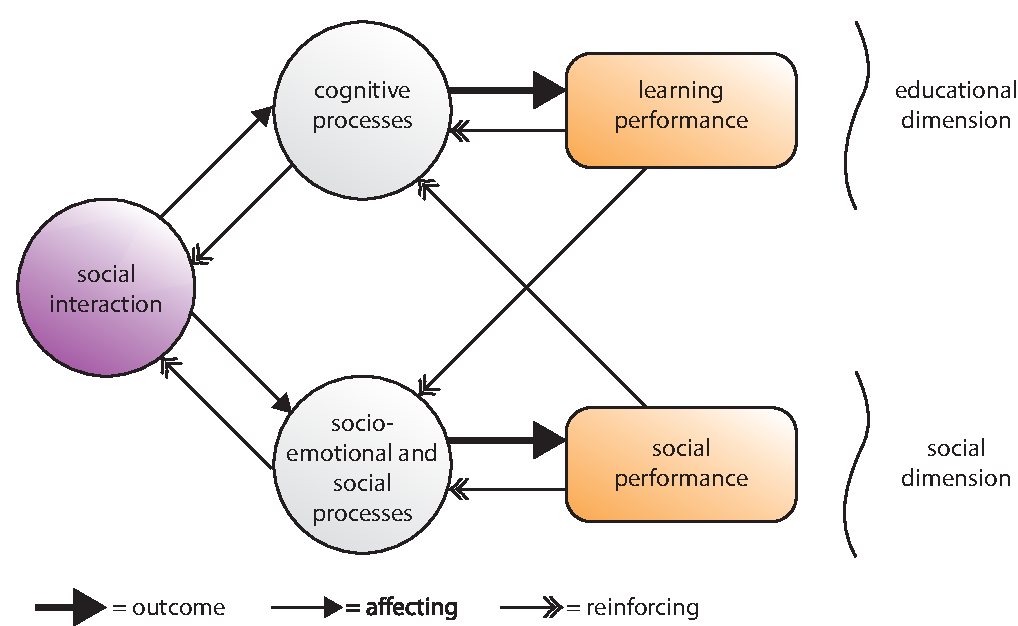
\includegraphics[width=0.7\textwidth]{images/ch2_SocialInt.pdf}
    \caption{A depiction of the role of social interaction for an individual, with two possible outcomes: social performance and learning performance - adapted from \cite{kreijns2003identifying}}
    \label{fig:ch2-rolesocial}
\end{figure}

Social interaction can be considered as the bond between cognitive processes and socio-emotional processes \citep{kreijns2003identifying}. The outcome of such interactions can be measured through social performance or learning performance, either of which can in turn reinforce the cognitive or socio-emotional processes taking place in an individual (Figure~\ref{fig:ch2-rolesocial}). This concept is supported through definitions of learning, which can be broken down into `affective' and `cognitive' learning (\citealp{bloom1956taxonomy}; this is further expanded on in Section~\ref{sec:background-learning}). Social interaction has the ability to influence both of these learning elements, and indeed \acrshort{hri} researchers have sought to do just this. Some researchers have focussed on the social behaviour of the robot with the aim of influencing cognitive processes \citep{kennedy2015higher,szafir2012pay}, whereas others have sought to influence the socio-emotional processes to a greater extent \citep{castellano2013towards}. 

Social interaction will rely in large part on the social cues used. Between humans, social cues used by teachers are often found to influence learning and a robot's ability to utilise similar cues could be an advantage over virtual technologies. If the cues are appropriate, then there is more likelihood of a fluid interaction and for the robot to have greater social presence. As such, the impact of social cues in \acrshort{hhi} will now be explored to provide a background for the motivation of manipulating robot social behaviour in the context of education and learning tasks. Where effects seen in the \acrshort{hhi} literature have been shown in \acrshort{hri} contexts, this will also be indicated.

%%%%%%%%%%%%%%%%%%%%%%%%%%%%%%%%%%%%%%%%%%%%%%%%%%%%%
\subsection{Gestures} \label{sec:background-gesture}
Gestures play an important role in teaching and learning \citep{kelly2008gesture, macedonia2012gestures}. Children are more likely to repeat the speech of a teacher if a matching (non-symbolic) gesture accompanies the speech when compared to the same speech without a gesture, but less likely with a mismatched gesture compared to no gesture \citep{goldin2005our, goldin1999teacher}. This basic recall is a first step towards learning. Furthermore, these studies show that children can use gestures in understanding problem-solving strategies, giving them the potential to learn both through problem solving and how to approach solving problems.

For young children, it has been suggested that gesture use (specifically symbolic gestures) can facilitate cognition \citep{goodwyn1998encouraging}; possibly because gestures can lighten cognitive load, lending more resources to memory tasks \citep{goldin2001explaining}. Indeed when children are slightly older (aged 8-10) gestures can help learning to `last' for longer, with correct answers in an algebra follow-up test four weeks after a learning session staying higher in a gesture and speech condition than in a speech only condition \citep{cook2008gesturing}. Equally, gestures made by children can be used to assess their learning \citep{goldin1992assessing}, with adults able to be more certain of their judgements of children's learning when their gestures matched their verbal explanation.

Such findings are reinforced in studies concerning instructional communication for learning, with children's performance improving more when given instructions with gestures as opposed to without in a symmetry recognition test \citep{valenzeno2003teachers}. These findings seem to have been partially replicated in \acrshort{hri}, with a robot utilising contingent gesturing leading to increased recall of material from a presentation \citep{szafir2012pay}. However, precisely how to use gestures to influence learning in \acrshort{hhi} is an open field with many questions still necessitating futher exploration \citep{roth2001gestures}; this is even more true for \acrshort{hri} where less work examining the use of gesture and learning has been conducted.

The use of hands seems to be particularly important. It is not just the orienting of attention, such as with a laser pointer, but the fact that the gesture is done with a hand that leads to an improvement in learning \citep{rumme2008gestures}. It has been shown that humans can accurately interpret pointing by a humanoid robot (an Aldebaran NAO), but that for best results, the arm on the side which the object to be pointed at should be used \citep{wang2014directing}. However, whether the hand of robot has the same attentional and learning impact as that of a human is not known. It has also been established that being present (as opposed to on video) does not affect how much attention gestures draw between humans \citep{gullberg2002visual}, but no such study comparing humans and robots could be found.

%%%%%%%%%%%%%%%%%%%%%%%%%%%%%%%%%%%%%%%%%%%%%%%%%%%%%
\subsection{Gaze} \label{sec:background-gaze}
From an early age, children use social cues such as eye gaze to help direct their learning. Despite social cues distracting briefly from the material to be learnt, infants learn more with gaze cues present than when their learning is not directed by such cues \citep{wu2010social}. These positive effects have also been successfully implemented in computational models \citep{yu2007unified}. Even at 15 months old, children have a tendency to use the gaze of a social interaction partner, instead of distracting and erroneous saliency cues for word learning associations \citep{houston2006use}. The power of gaze, or even just the eyes, in influencing behaviour is still observed in adults, with surprisingly strong results. For example, just an image of eyes near a donation point can increase charitable donations by almost 50\% \citep{powell2012eye}.

Selective processing of social cues for learning has far-reaching implications for \acrshort{hri}. Head movement alongside eye gaze can assist humans in responding to robot cues \citep{boucher2010facilitative}; use of this social cue could have advantages in learning. However, this has not been found in infants learning from robots, where they follow the gaze direction of both a robot and a human, but only the human gaze facilitated the learning of an object's appearance \citep{okumura2013power}. It was suggested that this could signify a disposition of infants to consider humans a superior source for learning. It remains to be seen whether this holds true for slightly older children, or with children more familiar with the concept of robots. Equally, this result could be a demonstration that humans process robot gaze in a cognitively different manner, as argued in \cite{admoni2011robot}.

College students who receive gaze at the start of each sentence when receiving verbal information can recall significantly more than those who receive no gaze \citep{sherwood1987facilitative}. This holds true for both simple and difficult material, for both genders. It is hypothesised that this is because the interaction feels more `intimate' and prevents mind-wandering whilst receiving the information. These findings have also been shown to occur with younger children, aged between 6 and 7 \citep{otteson1979effect}. Greater gaze from a storyteller led to increased recall from children when subsequently asked questions, compared to those in a lesser (but still some) gaze condition. This study reveals a trend towards possible interaction effects between the information content, gender and gaze, speculating that females are less affected by gaze than males when the material is more difficult.

Logically, it follows that using appropriate robot gaze towards a child might be beneficial for recall and learning. Work done in virtual environments demonstrates that caution must be used, as simply staring at a human interactant actually reduces their willingness to engage in mutual gaze, despite increased opportunity \citep{dalzel2011don}. It should be noted that this difference in mutual gaze did not actually translate to a difference in task performance, but this was hypothesised as being due to the relative simplicity of the task. A similar effect has been observed in human-robot interaction studies as well \citep{kennedy2015comparing, looije2012help}, where a tutoring robot received more gaze, which could theoretically be beneficial for the learning, but no learning differences were found.

Nevertheless, gaze can clearly have positive effects on learning \citep{otteson1979effect, sherwood1987facilitative, okumura2013power, yu2007unified}, but if it is not meaningful, or is too abundant then it can discourage mutual gaze, thereby limiting potentially positive effects \citep{dalzel2011don}. This remains a challenge, as it is not trivial to decide how much gaze is `just right', or precisely when a gaze fixation should be made by a robot.

%TODO incorporate Lee - 2015 - Gaze contingency from dropbox??

%%%%%%%%%%%%%%%%%%%%%%%%%%%%%%%%%%%%%%%%%%%%%%%%%%%%%
\subsection{Touch} \label{sec:background-touch}
Touch has been shown to lead to a positive affective state in \acrshort{hhi}, even with very short touches and when subjects were unaware of the touch \citep{fisher1976hands}. This positive response to touch has also been shown in \acrshort{hri}. When a robot offered an `unfair proposal' to participants with touch, their EEG response showed less negativity towards the robot than when the robot did not touch as they made the proposal \citep{fukuda2012midas}. To place this work in the context of educational interactions under consideration here, liking does not necessarily result in better learning, but there are indications that if students like an instructor more they will achieve more highly \citep{gurung2007looking}.

Touch has also been linked with compliance \citep{gueguen2002touch}, a useful tool for teachers when they need to influence students in order to get them to engage with lessons. The potential for utilising touch in \acrshort{hri} and educational contexts has previously been highlighted \citep{salter2006learning} but, as yet, remains underexplored. More generally, it has been demonstrated in several experiments that touch can influence perceptions of robots by humans. A robot initiating touch can encourage humans to see them more positively and to work for longer at a monotonous task \citep{shiomi2016touch}. However, \cite{cramer2009hug} emphasise that care is needed when incorporating behaviours such as touch in interactions as combined effects can lead to negative outcomes. Social cue combinations have also been found by \cite{chen2011touched} between touch and verbal warnings; these types of effects will be discussed further in Section~\ref{sec:background-sync}.

%%%%%%%%%%%%%%%%%%%%%%%%%%%%%%%%%%%%%%%%%%%%%%%%%%%%%
\subsection{Vocal Intonation} \label{sec:background-voice}
The voice that an agent uses can dictate how much they are liked and how hard humans try to understand the material they are presented with \citep{atkinson2005fostering}. Those who interacted with an agent who had a human voice preferred the agent and also did better in learning transfer tests when compared to those who interacted with the same agent with a machine-synthesised voice. The sound of a voice can have a significant impact on retention and transfer of a novel subject when presented through narration \citep{mayer2003social}. Retention is better when a voice has a `standard' (as opposed to foreign) accent and is human rather than machine-like, as well as being more likeable in both cases.

However, this result was found with college students and virtual agents. It has not been established whether this effect is also observed outside of this restricted demographic, nor whether specific embodiments of robots create expectations that violate these rules. For example, it may be less appropriate to have a deep male human voice when using a robot such as the Aldebaran Nao\footnote{\href{https://www.aldebaran.com/en/humanoid-robot/nao-robot}{https://www.aldebaran.com/en/humanoid-robot/nao-robot}} than a RoboThespian\footnote{\href{https://www.engineeredarts.co.uk/robothespian/}{https://www.engineeredarts.co.uk/robothespian/}}. It is suggested that a possible uncanny valley effect \citep{moore2012bayesian,mori2012uncanny} may occur, where participant expectations are violated when a human voice is played alongside a not-convincing-enough animated agent. An indication in this direction has been found with virtual agents, where participants preferred an animated agent with a machine-like voice and a non-animated agent with a human voice \citep{baylor2003effects}.

Vocal intensity can also be used to influence learning. Compliance, a factor in learning, can be increased through raising vocal intensity, as in \cite{remland1994influence}. This \acrshort{hhi} study was conducted in a public space where compliance was greatest when using a medium level of vocal intensity; around 70dB. It is likely that this level would need adjusting depending on the ambient noise in the space a robot tutor would be acting in, and how far from a student it would be. Vocal intensity has successfully been combined with gestures in a model which is based on \gls{nonverbalimm} to improve attention and recall of a human in an \acrshort{hri} presentation scenario \citep{szafir2012pay}. Whilst not confirming all of the results discussed in this section relating to vocal prosody, it certainly demonstrates that there is great potential for many of the same principles from \acrshort{hhi} being applied to \acrshort{hri}.

Interestingly, speech rate does not appear to have a significant impact on recall \citep{simonds2006effects}. This could potentially be explained by the capacity of humans for speech. The average human speech rate is 125-150 words per minute, but adults have twice as much cognitive capacity, being able to process speech at 250-300 words per minute \citep{fulford1992systematically}. This gives a broad scope for increasing speech rate without any great change in terms of the listener's cognitive processing. There is also a distinction between recall of spoken information and understanding, which may have a different outcome when speech rate is varied.

%%%%%%%%%%%%%%%%%%%%%%%%%%%%%%%%%%%%%%%%%%%%%%%%%%%%%
\subsection{Facial Expression} \label{sec:background-expression}
Human studies have shown that recognition of emotion from facial expression is used from a very young age to help understand social events and regulate social interactions \citep{tronick1989emotions,zarbatany1985social}. In an \acrshort{hhi} study examining the relationship between the social cues and cognitive learning across a number of different cultures it was found that alongside gaze and vocal prosody, smiling from the teacher was one of the more strongly correlated cues to student learning \citep{mccroskey1996nonverbal}. This result has also been replicated more recently \citep{velez2008relationship}, additionally showing the positive relationship between social cues and motivation (with facial expressions having a large effect size).

Experimental data from human-computer interaction (\acrshort{hci}) with an embodied conversational agent revealed no significant difference in recall of subjects when interacting with an agent which was either neutral, or able to express joy and anger \citep{becker2013affective}. Several reasons are put forward as to why this may have been the case, including a ceiling effect within the task, the amount each emotion was displayed, or that the facial expressions were simply ignored in favour of focussing on the task. As such, it is unclear whether the benefits of facial expression seen in \acrshort{hhi} will translate to \acrshort{hci} and \acrshort{hri}.

Despite the suggested impact of facial expressions on learning or motivation in \acrshort{hhi}, no data could be found regarding the impact of learning and facial expressions of robots. A possible explanation is that much of the research to-date regarding learning in \acrshort{hri} is performed with robots such as the Aldebaran NAO, Keepon, and Wakamaru which have largely non-manipulable faces. Due to the movement required in expressing facial emotion, the uncanny valley \citep{mori2012uncanny} could also be a current limitation for robots.

%TODO include Cameron 2015 Expressions (in dbox)?

%%%%%%%%%%%%%%%%%%%%%%%%%%%%%%%%%%%%%%%%%%%%%%%%%%%%%
\subsection{Proximity and Body Orientation} \label{sec:background-orientation}
The proximity between interactants is correlated to compliance effects \citep{peters2007gaining}. It is suggested that a distance of 1-2 feet (30-60cm) is optimally conducive to compliance between humans (from studies conducted in Western cultures; \citealp{segrin1993effects}), however whether this is the same for \acrshort{hri} has not been established. This is possibly because judging the physical proximity at which a robot should be from a student would not necessarily be as simple as a strict 1-2 feet rule. In human interactions, verbal feedback can modulate (positively and negatively) the proxemic impact on compliance \citep{greene1977effects}. In \acrshort{hri}, comfortable distances are dictated through the complex interplay of factors such as the size of the robot \citep{hiroi2011influence}, how much the robot gazes towards a human and how likeable they previously perceive the robot to be \citep{kim2014distance}.

Only about 60\% of people conform to the same proxemic social norms with robots as they do with people \citep{walters2005influence}. That being said, compliance effects have been seen in educational interactions between children and robots at a distance of about 2 feet (60cm), although this hasn't been compared against a control with closer or further distances \citep{kennedy2014children}. Additionally, it would appear that younger children have a smaller personal space, presumably due to their smaller size, so further work would need to be done for people of different sizes \citep{aiello1974development}.

Research conducted with a robot in a variety of task contexts show humans generally prefer the robot to be 0.46-1.22 metres away \citep{huettenrauch2006investigating}. However, it is warned that the dynamic nature of interaction with a robot should not necessarily be reduced to a simplistic rule. Indeed, the previous paragraph suggested the impact of variable robot appearance and behaviour, but there are also environmental and task factors to consider. For instance, if it is important to hear speech in a noisy environment, then it might be that a closer distance between interaction partners is more comfortable, when outside of these parameters it would usually not be.

Several design guidelines for robotic proximity are presented in \cite{takayama2009influences}. It is suggested that people who are familiar to the robot can be approached more closely, to direct gaze away from the face of a human as an approach is made, and to factor in the human's attitude towards robots when maintaining distance. The impact of human attitude towards robots is further supported experimentally in \cite{mumm2011proxemics} where the necessity of building rapport before increasing closeness is emphasised. This could be an important factor in tutoring in order to gain compliance.

Studies directly examining the impact of body orientation on learning could not be found; this is possibly due to the entanglement of body orientation with many other social cues. If not orientated to an interaction partner only limited eye gaze will be possible, gestures may be occluded and it may be more difficult to hear any speech. Nor could any studies be found studying the specific impact of co-located physical proximity on learning; most work considers co-located learning against distance learning (not co-located), but this then becomes about social presence rather than proxemics. Logically, it would seem reasonable that a middle-ground should be sought. The robot should not be too far away as then the student may struggle to perceive verbal instructions and non-verbal signals. If more compliance is required, then a closer distance should be sought. Further research is required to decide what is to be considered `too close' in specific scenarios, with humans of certain ages and certain robot sizes/designs; work such as \cite{rae2013influence, walters2005influence} provides a strong starting point in this direction.

%%%%%%%%%%%%%%%%%%%%%%%%%%%%%%%%%%%%%%%%%%%%%%%%%%%%%
\subsection{Verbal Content Cues} \label{sec:background-verbal}
Social aspects of the verbal content that a teacher uses can influence student learning \citep{gorham1988relationship,witt2004meta}. These social aspects can include: personalisation, discussion outside of lesson content, asking questions, revealing personal information, and the type of language used (possessive or not, e.g., `our' or `the'). Research has been done in \acrshort{hri} with a view to improving the bond between children and robots through some of these means \citep{belpaeme2012multimodal}, but often this is not in the context of educational interactions. The exploration of verbal cues has been explored from various angles in \acrshort{hri} with regards to human perception (for example, \citealp{andrist2013rhetorical}), but not so much in respect to learning outcomes. With children, it has been found that `off-activity talk' - dialogue with a robot which does not concern the task being completed - encourages compliance in a therapeutic setting \citep{kruijff2014oat}. Personalisation in therapeutic contexts has also been considered. Children were asked a number of questions about their preferences and the robot then mentioned these in an interaction, the children who interacted with a personalised robot enjoyed the interaction more, but subject numbers were too low for statistical comparisons \citep{henkemans2013using}.

When broadening to consider the impact of verbal content on learning in \acrshort{hhi} and other technology based fields (such as \acrshort{hci}), a much greater quantity of research exists. \cite{mayer2004personalization} found differences in learning when an animated character used language in an explanation to students that was conversational, compared to when it was more formal. This was a very subtle change, of just changing the word `the' to `your' throughout descriptions. Students retained equivalent information in both conditions, but could transfer their knowledge significantly better when the explanation had used the conversational (`your') style.

A summary of tens of studies which consider learning in response to variations in the cues described at the start of this section can be seen in \cite{witt2004meta}. All of these studies deal with \acrshort{hhi}, but have a mix of measures and subject matters. It is found that there are large correlations between greater use of the verbal cues and perceived student learning (\textit{r}=.49), however the cases where cognitive learning is actually measured reveals a much smaller correlation (\textit{r}=.06). Differences between these measurements will be discussed in greater detail in Section~\ref{sec:background-learning}. These findings suggest that verbal cues play a much smaller role in learning than nonverbal cues (which have almost 3 times as large a correlation in the same meta-analysis).

%%%%%%%%%%%%%%%%%%%%%%%%%%%%%%%%%%%%%%%%%%%%%%%%%%%%%
\section{Perspectives on Social Behaviour} \label{sec:background-sync}
Social cues do not occur in isolation, neither from other cues, nor from the environment and the interaction they are being used in. Behaviour is multimodal, and cues used must be congruent with other social cues being utilised in order to be interpreted correctly and efficiently. Social cues could be perceived as a single percept, which requires that cues be considered as an integrated whole \citep{zaki2013cue}. 

These concepts are exemplified experimentally by \cite{byrd2014gesturing} who further explored the conclusions drawn from studies such as those done by \cite{cook2008gesturing} regarding gestures and learning (discussed previously in Section~\ref{sec:background-gesture}). They found that when children did not copy eye movements accompanying gestures the lasting learning effect disappears. Similar results have been found elsewhere. In  \cite{langton2000mutual, langton2000you}, head gaze, gestures and spoken words were all used to direct attention. When any of the cues were incongruent (e.g., responses had to be made to head-gazes, whilst a pointing gesture was made in a different direction), interference effects were found, slowing down responses. If social cues are not synchronous and congruent then interactions will likely be impeded by this additional processing time.

In \acrshort{hri} there is often a tendency to manipulate only one behavioural cue at a time in order to tightly control experiments. This approach allows the findings to be directly attributed to the cue that is manipulated, but conclusions are often made which advise how this cue should be used without consideration for the larger context that this cue was used in. For example, if gestures are found to improve recall (as in \citealp{szafir2012pay}) when mutual gaze is often made, it is unclear if the same effect on recall would be observed if mutual gaze is no longer made. \cite{zaki2013cue} posits that perceptions (and subsequently outcomes) are a product of the combined gaze and gesture cues used, so the findings for gestures would depend on the gaze model used. Indeed, such interaction effects between behavioural cues have been found in \acrshort{hri} (previously discussed in Section~\ref{sec:background-touch}; \citealp{chen2011touched,cramer2009hug}).

Where larger scale manipulations have been made, some studies have sought to tease out the influence of particular cues in order to make more specific recommendations. \cite{huang2013modeling} use statistical techniques to derive the gestural predictors for interaction outcomes such as information recall. However, it is unclear how this could be re-implemented as a behaviour and whether the findings would remain should other social cues change. Not just the cues being used, but also their contingency can influence interactions. A robot which displays more contingent social cues, such as appropriate gaze and pointing gestures in response to a human, can elicit greater participation in an interaction \citep{lohan2012contingency}. When applied to an educational context, it is reasonable to suggest that greater participation will lead to an increase in learning \citep{anderson1975student}.

Based on the evidence put forward in this section, there is a need for further research in evaluating robot behaviour as a unified set of cues, i.e., as the product of a combination of social cues, rather than as separable cue elements additively forming a behaviour. The work in this thesis contributes to such research in Chapters~\ref{chap:socasoc}, \ref{chap:nviexperiment}, and \ref{chap:verbal}. As a consequence of this approach, conclusions will often not be drawn about specific social cues, but about sets of cues forming higher-level behaviours. This also means that analysis of robot behaviour needs to consider social cues in the context of one another; this challenge will be addressed in Section~\ref{sec:background-immediacy}.

Furthermore, evidence suggests that social behaviour will vary depending on the environment that interactions take place in \citep{ros2011child,salter2008going}. As such, if a study applied to a domain is to have ecological validity, then it ought to be conducted in the environment in which the interaction would actually take place in, or at a minimum with `experimental realism' \citep{berkowitz1982external}. In the case of educational interactions, this might mean a school, or a home, depending on the specific application. Conducting experiments in naturalistic environments, or `the Wild', introduces a number of methodological challenges \citep{ros2011child}, but they are worth the additional effort if the results have more ecological validity. Given the application of dyadic tutoring interactions being studied throughout this work, all experiments take place in children's schools.

%%%%%%%%%%%%%%%%%%%%%%%%%%%%%%%%%%%%%%%%%%%%%%%%%%%%%
\section{Approach to Teaching and Learning for this Thesis}\label{sec:background-learning}
It is important to note that throughout the work presented here, the focus is on the social behaviour of the robot, rather than on the higher level teaching strategy. This is necessitated through the focus on the research questions and scope laid out in Chapter~\ref{chap:intro}. Nonetheless, an understanding of definitions and processes of learning are required to use learning as a metric in studies, so these will be explored in this section with the goal of describing the position taken in the subsequent research presented. When considering the tutoring literature it is important to distinguish between different intended meanings of the term `learning'. Learning can be broken down into several different domains and stages, with various researchers attempting to provide a taxonomy of learning to formalise these concepts \citep{bloom1956taxonomy, krathwohl1964taxonomy}. Learning can also be approached in many different ways, with a variety of adopted perspectives determining how learning, and teaching, are carried out.

\cite{krathwohl2002revision} developed a revised taxonomy of educational objectives based on the original version by \cite{bloom1956taxonomy}. The aim of the original taxonomy was to provide not only a measurement tool for education, but also to provide a common language for communicating about learning and this is maintained in the revised version \cite{krathwohl2002revision}. This feature makes it ideally placed for use in defining learning for this thesis. In the revised taxonomy there are two dimensions: `cognitive process' and `knowledge'. Each dimension has several stages, which form a loose hierarchy (Figure~\ref{fig:learningtaxonomy}). 

\begin{figure}[ht]
    \centering
    \includegraphics[width=0.75\textwidth]{images/ch2_LearningTaxonomy.pdf}
    \caption{The revised educational objectives `Taxonomy Table' (adapted from \citealp{krathwohl2002revision}). Crosses indicate the areas focused on in studies throughout the research here, with the red cross signifying the intersection at which performance is most often measured.}
    \label{fig:learningtaxonomy}
\end{figure}

The knowledge dimension consists of \textit{factual}, \textit{conceptual}, \textit{procedural} and \textit{meta-cognitive} knowledge types. Briefly, these can be defined as follows \citep{krathwohl2002revision}:
\begin{itemize}
	\item \textit{Factual} - terminology or details required to work in a discipline
	\item \textit{Conceptual} - category, principle and generalisation knowledge
	\item \textit{Procedural} - skill, algorithm, technique and method knowledge for subject-specific tasks
	\item \textit{Meta-cognitive} - knowledge of cognitive processes and one's own cognition
\end{itemize}

For the work in this thesis, the goal is for children to learn a new skill and to generalise this skill to novel stimuli. As such, this addresses the following cognitive educational objectives: \textit{remember}, \textit{understand}, and \textit{apply}. \textit{Apply} is at the highest level of the hierarchy of these, and so this will constitute the primary evaluation of the learning: to apply requires the children to have remembered and understood. Therefore, to assess the \textit{apply} stage also implicitly assesses the \textit{remember} and \textit{understand} stages. \cite{mayer2002rote} discusses the importance of learning going beyond the \textit{remember} stage and to be able to transfer any new knowledge to new problems.

Of course, when measuring the application of skills that the children have acquired, the actual measurement is not necessarily of \textit{learning}, but of \textit{performance} in the task \citep{mikulas1977learning}. Task performance may rely not just on learning but also on several other factors such as motivation, fatigue, and so on. Due to complexities in separating learning from other factors in task performance \citep{mikulas1977learning}, for the purposes of the work here, it will be assumed that changes in task performance reflect learning to at least some degree if experimental factors remain constant. Throughout, the aim is to influence learning, rather than task performance as task performance can be improved through mere repetition, whereas learning involves some aspect of knowledge transfer to solve previously unseen problems (which has the potential to be more useful).

An important distinction lies in the difference between `affective learning', `cognitive learning' and `perceived learning', which are commonly presented in the \gls{immediacy} literature \citep{witt2004meta}. \textit{Affective} learning considers constructs such as attitudes, values and motivation \citep{krathwohl1964taxonomy}. \textit{Cognitive} learning consists of the elements discussed in \cite{krathwohl2002revision} and shown in Figure \ref{fig:learningtaxonomy}; these are typically topic specific knowledge and skills. \textit{Perceived} learning is a measure of how much students believe they have learnt, or how confident they are in what they have learnt, such as in \cite{gorham1988relationship}.

With perceived learning, students are asked how much they believe they have learnt, often on a Likert scale, and this is used as the learning measure. This approach is commonly justified through precedence, for example in \cite{butland1992teacher}, but does have some basis in evidence \citep{perry2007scholarship}. This measure has the advantage of being applicable across multiple domains and learning objectives. However, there are challenges in using self-reporting measures of this nature with children \citep{borgers2000children}, and some journals question the correlation between perceived and actual learning, refusing data based on self-assessments of learning \citep{dipiro2010student}. Due to the self-reporting nature of affective learning, the same challenges as perceived learning are faced when surveying children \citep{borgers2000children}. However, cognitive learning often has clear and quantitative means of measurement, lending itself well to a measurable outcome of interactions with robots. For this reason, the studies in this thesis focus on measuring cognitive learning.

%%%%%%%%%%%%%%%%%%%%%%%%%%%%%%%%%%%%%%%%%%%%%%%%%%%%%
\section{Robots as Educators}\label{sec:background-robottutors}
This section will build upon the literature exploring embodiment and social presence effects of robots on learning and task performance introduced in Section \ref{sec:background-tutor} by considering the literature studying the effects of robot behaviour on learning and social responses in \acrshort{hri} in educational contexts. It should be noted that the focus is on robots used to deliver some aspect of teaching content (robots as educators), rather than robots used as a teaching platform (educational robotics). Section \ref{sec:background-behave} showed that if the social behaviour of an agent can be improved then the social presence will increase and interaction outcomes should improve further, but it is unclear how social behaviour should be implemented to achieve such aims. This has resulted in researchers exploring various aspects of robot social behaviour and attempting to measure the outcomes of interactions in educational contexts, but a complex picture is emerging. This section will introduce literature from \acrshort{hri} with a view to establishing the state of the field in using robots to educate children. Particular attention will be paid to work involving children, measuring cognitive learning gains, as this closely relates to the scenario in this thesis.

\subsection{Roles of Robots in Education}
Robots can adopt a variety of roles when interacting with children in learning environments. These roles have been the subject of various research endeavours, which will be summarised here. Robots have been used as peers for children. This approach has the advantage that the robot can be programmed with less knowledge than the child, so can convincingly play this role in the way that their human class teachers cannot (and nor can their peers if they are lower ability within their cohort; \citealp{kennedy2016heart}). A robot was employed as a less-able peer to help improve children's handwriting, with promising preliminary results \citep{hood2015children}. In a similar methodology, \cite{tanaka2012children} use a robot which requires care (a care-receiving robot) from children. The aim is for the children to learn by teaching, and their results show that children's vocabulary acquisition is indeed higher in sessions with the robot than without the robot. The children also retain this vocabulary a number of days later. This work was conducted with the Aldebaran NAO, and more recent efforts have applied the same principle to the Aldebaran Pepper, with results forthcoming \citep{tanaka2015pepper}. It should be noted that this work does not compare a care-receiving robot to a non-care-receiving robot, so no conclusion can currently be drawn as to whether this technique holds advantages over other methods of tutoring. Other work with forthcoming results also aim to employ robots in a peer role \cite{kory2014storytelling}.

Other researchers have employed robots in roles closer to teaching assistants. \cite{kanda2004interactive} found learning of a language was related to time interacting with a robot, however, this was only true for the second week of a 2 week study. Novelty effects may account for the lack of significance between interaction and learning in the first week, although the study was not designed to attempt to teach in an optimal manner, but to investigate the possibility of maintaining relationships with robots on a daily basis. A more controlled study by \cite{alemi2014employing} found that using a a robot to supplement teaching over a 5 week period led to significant learning increases when compared to the same material being covered with a human teacher without a robot. This is strong evidence for the positive impact that robots can have in education.

Robots have also been used in a tutoring role. As previously discussed in Section \ref{sec:background-behave}, a Keepon robot was used as a tutor in a logical puzzle solving task with adults to explore embodiment effects \citep{leyzberg2012physical}. This work was extended further to study the teaching strategy that the tutor adopted by personalising when hints were delivered. It was found that when lessons were personalised based on an assessment of human skill, significant improvement was found in puzzle solving times when compared to a no lesson or randomized lesson control group \citep{leyzberg2014personalizing}. More in-depth exploration of such personalisation behaviours for robot tutors is also planned by other researchers \citep{charisi2015towards}.

Based on these different approaches, some researchers have attempted to establish the most effective role for robots to assume in an interaction. \cite{blancas2015effects} found no significant differences in performance of humans whether taught history by a teacher or a peer robot. Their conditions were operationalised through changes in verbal content and nonverbal behaviour such as gestures. However, their study was conducted with adults, and the teaching element only lasted for 2.5 minutes with unidirectional interaction (the robot read a script to the human). Whether these findings would persist when transferred to interactions with children, over longer periods of time, and with a greater degree of interaction, remains to be seen. \cite{zaga2015effect} also explore this question, comparing a robot as a peer with a robot as a tutor, when supervising pairs of children completing a logical puzzle. It was found that children performed better with the peer robot and looked at the peer robot more, but prior ability was not controlled for and subject numbers were relatively low (5 pairs per condition). \cite{diyas2016evaluating} does not observe conclusive differences in response to different robot roles (`peer' vs `teacher') when manipulating verbal behaviour. This therefore seems to remain an open question, but the best role for the robot may well depend on its morphology as this may set particular expectations (a large, complex robot may not make a convincing peer in the same way a NAO might, for example).

\subsection{Robot Behaviour in Educational Interactions}
Aspects of a robot's non-verbal behaviour have been investigated in one-on-one tutoring scenarios with mixed results. \cite{herberg2015robot} found that the \acrshort{hhi} literature would predict an increase in learning performance with increased gaze of a robot towards a pupil, but the opposite was observed. An Aldebaran NAO would either look towards or away from a child while they completed a worksheet based on material they had learnt from the robot. Additional gaze towards the child was predicted to increase performance. This was not found to be the case, but a potential confound of robot movement \textit{vs} non-movement may have played a role in the behaviour of the children. However, \cite{saerbeck2010expressive} varied socially supportive behaviours of a robot in a novel second language learning scenario. These behaviours included gestures, verbal utterances and emotional expressions. Children learnt significantly more when the robot displayed these socially supportive behaviours.

The impact on child learning of verbal aspects of robot behaviour have also been investigated. \cite{gordon2015curiosity} developed robot behaviours to promote curiosity in children with the ultimate aim of increased learning. Whilst the children were reciprocal in their curiosity, their learning did not increase as the \acrshort{hhi} literature would predict. \cite{kanda2012children} compared a `social' robot to a `non-social' robot (operationalised through verbal utterances to children when they are completing a task). Children showed a preference for the social robot, but no learning differences were found.

Methodological complications meant that in a study by \cite{short2014train} it is unclear whether children learnt about nutrition from a robot. The study attempted a longer-term interaction protocol, with 6 sessions. Response time for choosing food was used a metric, but the questions also became progressively more difficult, which acted as a confound to the chosen indication for learning. As part of the same project, but with a different educational focus (mathematics tutoring), \cite{ramachandran2016shaping} used a robot to shape requests that children made for help. They found that a robot which shaped sub-optimal help strategies from children led to the children modifying their behaviour and learning more when compared to a control condition, where the robot did not shape sub-optimal strategies. It has also been suggested that children are more likely to ask for help from robots in educational interactions as there is less of a social stigma involved with doing so when compared to asking other humans for help \citep{howley2014effects}.

Ultimately, it is a difficult task to present a coherent overview of the current state of research in the child-robot interaction (\acrshort{chri}) educational domain with many results appearing to contradict one another, or not being comparable due to the difference in learning task or behavioural context. More researchers are now using the same robotic platforms and peripheral hardware than before (quite commonly the Aldebaran NAO or DragonBot with a large touchscreen, e.g., \citealp{baxter2012touchscreen}), but there remain few other similarities between studies. Behaviour of various elements of the system are reported alongside learning outcomes, but it is difficult to translate from these descriptions to something which can be compared between studies. As such, it becomes almost impossible to determine if differing results between studies (and discrepancies with \acrshort{hhi} predictions) are due to differences in robot behaviour, the study population, other contextual factors, or indeed a combination of all three. It is apparent that a characterisation of the robot social behaviour would help to clarify the differences between studies and provide a means by which certain factors could be accounted for in analysis; this will be explored in the following section, and demonstrated throughout the experiment-focussed chapters of this thesis (Chapters \ref{chap:embodiment}-\ref{chap:verbal}).

% note: this paragraph was promised in the intro, so needs to exist in some form (distinction between 1 and 2 specified below)
Prior work reveals two main avenues of exploration in \acrshort{hri} for education: \textit{(1)} study of different teaching strategies (e.g., \citealp{leyzberg2014personalizing,ramachandran2016shaping}), and \textit{(2)} study of the effects of social behaviour/presence (e.g., \citealp{kanda2004interactive,saerbeck2010expressive,zaga2015effect}). One of the main distinctions between the two approaches is in the nature of the specificity of findings. Manipulations to the teaching strategies are specific to the particular educational topic of focus, whereas the behavioural findings could theoretically be applied to other topics. It is not clear from \acrshort{hri} findings that this transfer still produces the same outcomes, but \acrshort{hhi} literature suggests that it would (as discussed in Section \ref{sec:background-behave}). However, there are few clear guidelines on how to operationalise robot behaviour to optimise child learning; this is an area that this thesis will contribute to.

%%%%%%%%%%%%%%%%%%%%%%%%%%%%%%%%%%%%%%%%%%%%%%%%%%%%%
\section{Characterising Social Behaviour} \label{sec:background-immediacy}
To allow researchers to make clearer comparisons between studies and across contexts, a metric (or set thereof) to characterise the social behaviour of a robot is desirable. Various metrics have been used before in \acrshort{hri} and some of these will be introduced here. For the purposes of the research conducted as part of this thesis it is desirable to have a metric which is appropriate for use with children.

Retrospective video coding has been used in several \acrshort{hri} studies as a means of measuring differences in human behavioural responses to robots, for example \citep{kennedy2015comparing, moshkina2014social, tanaka2012children}. However, for cross-context and cross-study comparisons it is important for the metric to be holistic in its characterisation of the social behaviour so that all social cues are considered in the context of one another. For example, when studying gaze, it is important to know whether gestures are occurring at the same time, and so on, as this could influence human perception and experimental findings \citep{zaki2013cue}. This should be accounted for within the metric for characterisation, and so manual video coding is not well suited for this kind of approach due to the time intensive requirements of such analysis.

The Godspeed questionnaire series developed by \cite{bartneck2009godspeed} has been used in many \acrshort{hri} studies to measure users' perception of robots \citep{bartneck2009does,ham2011influence}. The animacy and anthropomorphism elements of the scale in particular consider the social behaviour and perception of the robot. However, it is not particularly suited to use with children due to the language level (i.e., use of words such as `stagnant', `organic', `apathetic'). It may also be that the questionnaire would measure aspects of the robot not directly related to social behaviour as it is asking about more general perceptions. Whilst this could be of use in many studies, for the aim of characterising social behaviour in the case here, these aspects prevent suitable application.

Immediacy was introduced by \cite{mehrabian1968some} and is defined as the `psychological availability' of an interaction partner. Immediacy can be broken into nonverbal and verbal aspects. Several versions of surveys have been developed and validated for measuring the \gls{nonverbalimm} of adults \citep{richmond2003development}. Surveys have also been developed for \gls{verbalimm} \citep{gorham1988relationship}, but their ability to measure precisely the concept of \gls{verbalimm} remains the subject of debate \citep{robinson1995validity}. Both verbal and nonverbal measures consider observed overt behaviour more than, but not excluding, perceptions. Immediacy has recently been used in \acrshort{hri} as a means of motivating robot behaviour manipulations \citep{szafir2012pay} and characterising social behaviour \citep{kennedy2015higher}. Whilst the \gls{immediacy} surveys are not designed for use with children, the consideration of only overt behaviour allows a researcher to simplify the language to an appropriate level, which is not necessary possible with more abstract concepts (such as `organic' seen in the Godspeed series).

BEHAVE \citep{joosse2011behave} and BEHAVE-II \citep{joosse2013behave} are measures for assessing users' attitudinal and behavioural responses to a social robot. These measures in part utilise concepts of \gls{nonverbalimm}, but combine them with more extensive questioning of personal space/proxemics, and observations of emotion. Whilst these measures are designed for measuring user behaviour rather than robot behaviour, it could be reasonable to manipulate the questions to make them robot-centric. However, the perception and interpretation of a robot's emotion (if existent) by children would not necessarily be trivial and the proxemic behaviour questions have less relevance when the interactants have fairly static locations as in the interactions considered in this work.

%%%%%%%%%%%%%%%%%%%%%%%%%%%%%%%%%%%%%%%%%%%%%%%%%%%%%
\section{Nonverbal and Verbal Immediacy} \label{sec:lit-immediacy}
As stated previously, immediacy was introduced by \citet{mehrabian1968some} and is defined as the `psychological availability' of an interaction partner. More generally, this is ``the extent to which communication behaviours enhance closeness to and nonverbal interaction with another'' \citep{mehrabian1968some}. A number of specific social cues are used (touching, distance, forward lean, eye contact, and body orientation) to form part of the measure for this concept, which were later utilised by researchers that sought to create and validate measuring instruments for immediacy, e.g., \citet{richmond2003development}. 

Immediacy was selected as the most appropriate metric for characterising robot social behaviour throughout the work presented here. There is a consensus on the instruments used to measure \gls{nonverbalimm} (whereas this is less clear for \gls{verbalimm}) and it is also transparent in terms of how participants are judging the robot. The Godspeed questionnaire is a useful tool for gathering perceptions, but \gls{nonverbalimm} focusses on accounting for overt social behaviour and so it is ideal given the aim of trying to characterise social behaviour (often with children). Immediacy has undergone extensive evaluation and validation in human-human studies. This brings with it the advantages that it can be considered to be reliable, and that it can tie findings to other literature exploring \gls{nonverbalimm} and \gls{learning}. The \gls{immediacy} metric as adapted and applied in this thesis will be discussed in greater detail in Chapter~\ref{chap:method}, while a more general introduction and background to the concept will be provided here.

\subsection{Application in Human-Human Interaction}
A reasonable volume of data already exists for studies considering immediacy, with over 80 studies (and \textit{N} nearly 25,000) from its inception to 2001 \citep{witt2004meta}, and more since. This provides a context for NVI findings in HRI scenarios and a firm grounding in the human-human literature from which roboticists can draw. It has found extensive application in educational research, most often in university lecture scenarios \citep{witt2004meta}. This application to education is particularly relevant given the domain of this thesis, although the target population here is young children rather than university students.

When used in studies between humans, the correlation with measured cognitive learning gains is only moderate, however relatively few studies have used experimental measures; most have used perceived learning, which has a particularly strong correlation with teacher immediacy \citep{witt2004meta}. It has been experimentally found that perceived learning and actual recall are moderately correlated in such contexts \citep{chesebro2000relationship}, so whilst perceived learning is not as strong as measuring actual learning, it can at least be used as an indication of the nature of relationships. A positive correlation between nonverbal immediacy and perceived cognitive learning has been validated across several cultures, including the United States, Puerto Rico, Finland and Australia \citep{mccroskey1996nonverbal}. From this, \citet{mccroskey1996nonverbal} postulate that expectation of immediacy plays a key role in how cues are interpreted, presenting opportunities for high immediacy teaching to have a strong positive impact in generally low immediacy cultures, but a negative impact for low immediacy teaching in high immediacy cultures. A similar suggestion relating to the use of robot social cues in teaching contexts has also been raised in HRI \citep{kennedy2015less}.

% distinction between verbal and nonverbal
Immediacy can be broken down into verbal and nonverbal aspects. Nonverbal immediacy measures consider specific social cues: gaze, gesture, body posture, proximity, etc. However, verbal immediacy is less clearly defined as a measure \citep{robinson1995validity}. The verbal immediacy metric proposed by \citet{gorham1988relationship} includes various personalisation aspects such as using an interacting partners' name, along with aspects of familiarity, such as revealing personal information. Whilst the nonverbal immediacy scale is a general characterisation of an individuals' social behaviour, this proposed verbal immediacy scale is specifically designed for educational environments, with items such as ``the instructor gets into conversations with individual students before or after class'' \citep{gorham1988relationship}. The implications of this in the context of this thesis are discussed in Section~\ref{sec:method-nvi}.

Both verbal and nonverbal immediacy behaviours have been shown to lead to an increase in motivation and, in turn, student learning \citep{christensen1998linear, christophel1990relationships}. In some cases, such as in a task to recall contents of a lecture \citep{chesebro2003effects}, cognitive learning gains are not found, but affect for the instructor and material increases when the instructor is judged to have higher nonverbal immediacy. However, there are other examples demonstrating a link between more nonverbal immediacy and increased recall \citep{goodboy2009effects, witt2001experimental}. An extensive review of the potential benefits of immediacy (both verbal and nonverbal) can be seen in \citet{chesebro1998relationship}. There are suggestions that the relationship may not be wholly linear in nature \citep{comstock1995food, witt2006influence}, but instead an inverted U shape. This would suggest that if social behaviour is too high in nonverbal immediacy then it could start to become detrimental to learning. As such, it remains unclear how immediacy should be implemented for social robots, which this thesis aims, in part, to make a contribution towards. This lack of clarity in findings between humans also creates a limitation in that it makes it more challenging to identify whether findings are a property of using robots, or a property of nonverbal immediacy itself.

\subsection{Application in Human-Robot Interaction}
Nonverbal immediacy has been studied only briefly in HRI contexts before, and besides the work later in this thesis, verbal immediacy does not seem to have been applied in an HRI context. \citet{szafir2012pay} use nonverbal immediacy as a means of motivating and evaluating robot behaviour during a recall task with adults. In line with literature studying nonverbal immediacy with humans, they find that as immediacy increases, so does recall. The adults were also able to notice when the nonverbal immediacy of the robot had increased, confirming that adults are sensitive to such cues in robots. Nonverbal immediacy concepts have also been used by the same research group to motivate behavioural manipulations for persuasive robots \citep{chidambaram2012designing}. However, it should be noted that it doesn't appear that a complete nonverbal immediacy questionnaire was used in either of the studies. Finally, nonverbal immediacy has recently been proposed for use in HRI studies to motivate exploring the perception of a robot when posture and nodding behaviour is varied \citep{jeong2015interested}.

\subsection{Measuring Immediacy}
Several versions of surveys have been developed and validated for measuring the nonverbal immediacy of adults \citep{richmond2003development}. Surveys have also been developed for verbal immediacy \citep{gorham1988relationship}, but their ability to measure precisely the concept of verbal immediacy remains the subject of debate. \citet{robinson1995validity} highlight the lack of negatively worded items and suggest that this inhibits the face validity of the survey. The construct validity is further called into question given the low correlation between verbal immediacy, nonverbal immediacy and affect towards an instructor using data from an experiment \citep{robinson1995validity}.

The nonverbal immediacy measure proposed by \citet{richmond2003development} has generally excellent face validity due to the fact that it contains items that explicitly explore the nonverbal behaviours included in the definition of the concept provided by \citet{mehrabian1968some}. However, there are also two items that are less clearly directly attributable to specific social behaviour cues, and could instead could be considered a more subjective rating, for example ``Looks bland or neutral when talking to people''. It is unclear how looking `bland' should be interpreted. This problem is exacerbated in the version of the questionnaire developed as part of this thesis, where the language was modified for children.

\citet{wilson2007immediacy} have sought to validate the use of the immediacy measure proposed by \citet{gorham1988relationship}. This measure was proposed as a verbal immediacy measure, but also includes 5 items from the nonverbal immediacy measure (all positively worded, avoiding the more subjective items referred to in the previous paragraph). It was found that the immediacy ratings (both verbal and nonverbal) were correlated to perceptions of instructor effectiveness and that a factor analysis revealed both aspects are valid measures of immediacy (in both face and construct validity). The study was conducted with 44 instructors and 1572 participants, so this provides some reassurance that the surveys do indeed measure the concept of immediacy, although these findings are contrary to those of \citet{robinson1995validity}. Additionally, not all nonverbal immediacy items were included. This unclear validity is a potential limitation of the measure, and more so, the adaptation used here where items with questionable face validity become difficult to interpret when modifying the language for children (described in Section~\ref{sec:method-nvi}).

Perceptions of immediacy have been validated through physical manipulation of some of the social cues, specifically eye gaze and proximity, in order to ensure that the phenomenon works in practice and is not a product of affect or bias in survey responses \citep{kelley1988effects}. It was indeed found that the physical manipulations that were made which would lead to a higher immediacy score (standing closer and providing more eye gaze) did lead to increased short-term recall of information. While there is clearly a difference between recall and learning, recall of information is a promising first step to acquiring new understanding and skills. These results were hypothesised to exist in the other immediacy behaviours (such as gestures) as well.

Overall, the link between teacher immediacy and student learning is hypothesised to be a positive one, as reflected in the meta review by \cite{witt2004meta} and many studies, e.g., \citet{christensen1998linear,comstock1995food,mccroskey1996nonverbal}. Despite some debate about the validity of immediacy, it is particularly appealing for HRI as the measures can be used as lists of overt social behaviours that robot behaviour designers can manipulate. To the authors' knowledge, no other metric for social behaviour currently provides this relatively low-level guide for behaviour implementation, while simultaneously offering a means of characterising social behaviour and verifying behavioural manipulations.

%%%%%%%%%%%%%%%%%%%%%%%%%%%%%%%%%%%%%%%%%%%%%%%%%%%%%
\section{Summary}\label{sec:background-summary}
This chapter has described the motivation for creating robot tutors, and provided a definition of learning for this thesis for clarity and to focus the scope of the work. Literature from both human-human studies and human-robot studies which led to the research questions formulated in Chapter~\ref{chap:intro} was discussed. Human-human studies reveal that social behaviour can positively influence learning, but human-robot studies present a more complex picture. Differences in methodologies and behaviours mean that it is unclear precisely how a robot should behave in educational interactions, and makes a measure for robot social behaviour desirable. A review of social behaviour metrics revealed that \textit{\gls{immediacy}} could be applied to \acrshort{hri} to characterise robot social behaviour, and possibly also to tie findings to the broader \gls{immediacy} literature examining human learning in response to different social behaviours.